% ============================================================
% Campus Resource Hub — Final Project Report
% Format: Northern University Bangladesh, Dept. of CSE
% ------------------------------------------------------------
% HOW TO USE:
%  1. Fill in your details in the "STUDENT / SUPERVISOR INFO"
%     block just below.
%  2. Put figures (PNG screenshots) in the figures/ folder with
%     the file names referenced in each \reportfig call. Missing
%     figures show a labelled placeholder box, so the document
%     always compiles.
%  3. Compile with XeLaTeX / Tectonic, or upload to Overleaf.
% ============================================================
\documentclass[12pt,a4paper]{report}

% ---------- STUDENT / SUPERVISOR INFO (EDIT ME) -------------
\newcommand{\ProjectTitle}{Campus Resource Hub: A Centralized Web Platform for Academic Resource Sharing with AI-Powered Moderation and Semantic Search}
\newcommand{\StudentAName}{Akib Rayhan}
\newcommand{\StudentAID}{42230200858}
\newcommand{\StudentBName}{Rakibul Hasan}
\newcommand{\StudentBID}{42230200859}
\newcommand{\StudentCName}{Mahdi Hasan}
\newcommand{\StudentCID}{42230200717}
\newcommand{\SupervisorName}{Tanmoy Mazumder}
\newcommand{\SupervisorRank}{Lecturer}
\newcommand{\DeptHeadName}{Md.\ Raihan-Ul-Masood}
\newcommand{\SubmissionDate}{July 2026}
% -------------------------------------------------------------

\usepackage[a4paper,left=1.25in,right=1in,top=1in,bottom=1in]{geometry}
\usepackage{newtxtext,newtxmath}          % Times-like font
\usepackage{setspace}
\usepackage{graphicx}
\usepackage{booktabs}
\usepackage{array}
\usepackage{longtable}
\usepackage{caption}
\usepackage{enumitem}
\usepackage{titlesec}
\usepackage{xcolor}
\usepackage{tikz}
\usetikzlibrary{shapes.geometric,arrows.meta,positioning,fit}
\usepackage[hidelinks]{hyperref}

\onehalfspacing
\setlength{\parindent}{0pt}
\setlength{\parskip}{6pt}

% ---------- Chapter / section heading style ------------------
\titleformat{\chapter}[block]
  {\centering\bfseries\Large}{Chapter \thechapter:}{0.4em}{}
\titlespacing*{\chapter}{0pt}{-20pt}{18pt}
\titleformat{\section}{\bfseries\large}{\thesection}{0.5em}{}
\titleformat{\subsection}{\bfseries\normalsize}{\thesubsection}{0.5em}{}

% Front-matter unnumbered heading
\newcommand{\frontheading}[1]{%
  \begin{center}\textbf{\Large #1}\end{center}\vspace{10pt}}

% ---------- Figure helper: placeholder if file missing -------
\newcommand{\reportfig}[4][1.0]{%
  \begin{figure}[htbp]
    \centering
    \IfFileExists{figures/#2}%
      {\fbox{\includegraphics[width=#1\textwidth]{figures/#2}}}%
      {\fbox{\parbox[c][5.5cm][c]{0.8\textwidth}{\centering
        \textit{Screenshot placeholder}\\[4pt]
        (add \texttt{figures/#2})}}}
    \caption{#3}
    \label{#4}
  \end{figure}}

\begin{document}

% ============================================================
% COVER PAGE
% ============================================================
\begin{titlepage}
  \begin{center}
    {\LARGE\bfseries Campus Resource Hub:\\
      A Centralized Web Platform for Academic\\
      Resource Sharing with AI-Powered\\
      Moderation and Semantic Search\par}
    \vspace{1.2cm}

    {\large Submitted By}\\[10pt]
    {\large \StudentAName}\\
    {\large ID: \StudentAID}\\[8pt]
    {\large \StudentBName}\\
    {\large ID: \StudentBID}\\[8pt]
    {\large \StudentCName}\\
    {\large ID: \StudentCID}\\[8pt]
    \vspace{0.8cm}

    {\large A Project Report Submitted in Partial Fulfillment of the
      Requirements for the Degree of Bachelor of Science in Computer
      Science \& Engineering\par}
    \vspace{0.9cm}

    \IfFileExists{figures/university-logo.png}%
      {
\includegraphics[width=3.4cm]{figures/university-logo.png}}%
      {\fbox{\parbox[c][3.5cm][c]{4cm}{\centering\textit{University\\logo}}}}
    \vspace{0.9cm}

    {\large\bfseries DEPARTMENT OF COMPUTER SCIENCE AND ENGINEERING\\
      NORTHERN UNIVERSITY BANGLADESH\par}
    \vspace{0.7cm}
    {\large \SubmissionDate}
  \end{center}
\end{titlepage}

% ============================================================
% FRONT MATTER
% ============================================================
\pagenumbering{roman}

% ---------------- APPROVAL ----------------------------------
\frontheading{APPROVAL}
The Project Report ``\ProjectTitle'' submitted by \StudentAName{}
ID: \StudentAID, \StudentBName{} ID: \StudentBID, \StudentCName{}
ID: \StudentCID{} to the Department of Computer Science and
Engineering, Northern University Bangladesh, has been accepted as
satisfactory for the partial fulfillment of the requirement for the
degree of Bachelor of Science in Computer Science and Engineering and
approved as to its style and contents.

\vspace{1.4cm}
\underline{Board of Examiners:}

\vspace{0.8cm}
1.\ \SupervisorName \hfill (Supervisor)

\vspace{1.6cm}
2. \hfill (Examiner)

\vspace{1.6cm}
3. \hfill (Examiner)

\vfill
\begin{center}
  \rule{6cm}{0.4pt}\\
  \DeptHeadName\\
  Associate Professor \& Head\\
  Department of Computer Science \& Engineering\\
  Northern University Bangladesh
\end{center}
\clearpage

% ---------------- DECLARATION --------------------------------
\frontheading{DECLARATION}
We hereby declare that the work presented in this project report is
the outcome of the investigation performed by us under the
supervision of \SupervisorName, \SupervisorRank, Department of
Computer Science \& Engineering, Northern University Bangladesh. We
also declare that no part of this project has been or is being
submitted elsewhere for the award of any degree or diploma.

\vspace{1.4cm}
\begin{center}
  Signature
  \vspace{1.2cm}

  \makebox[0.5\textwidth]{\dotfill}\\
  \StudentAName\\
  ID: \StudentAID
  \vspace{1.2cm}

  \makebox[0.5\textwidth]{\dotfill}\\
  \StudentBName\\
  ID: \StudentBID
  \vspace{1.2cm}

  \makebox[0.5\textwidth]{\dotfill}\\
  \StudentCName\\
  ID: \StudentCID
\end{center}
\clearpage

% ---------------- ABSTRACT -----------------------------------
\frontheading{ABSTRACT}
This project presents the design and implementation of
\textit{Campus Resource Hub}, a centralized full-stack web platform
that brings academic resource sharing, campus events, clubs,
lost-and-found services, announcements, and real-time communication
into a single system for a university community. The platform is
built on the MERN-style stack: a React single-page application on
the frontend and a Node.js/Express REST API with MongoDB on the
backend. Students can upload and download categorized study
materials (PDF, DOCX, PPTX, XLSX, and images), which pass through an
automated AI content-safety scan; unsafe, partially inspected, or
provider-unavailable uploads enter a human moderation workflow before
publication. The system implements secure email-OTP--verified
registration, JWT-based session management, and three-tier
role-based access control (student, moderator, administrator).
Real-time private and group messaging is provided through
Socket.io with delivery and seen receipts, and an event scheduler
supports capacity-aware RSVP management. A distinctive feature of
the platform is its semantic search subsystem: every published item
is converted into a 384-dimensional multilingual sentence embedding
and indexed in MongoDB Atlas Vector Search, enabling an AI assistant
to answer natural-language questions about campus content with
streamed responses. Files are stored in Cloudinary, and the system
is deployed on cloud infrastructure at zero recurring cost. Testing
shows the current free-tier deployment comfortably serves a
department-scale user base of 50--100 concurrent active users, with
a clear and inexpensive upgrade path to campus scale. The result is
a practical, secure, and extensible digital campus platform that
reduces information fragmentation and modernizes day-to-day academic
collaboration.
\clearpage

% ---------------- ACKNOWLEDGEMENT ----------------------------
\frontheading{ACKNOWLEDGEMENT}
First, we would like to show gratitude to almighty God, the most
merciful, for bestowing His blessings on us in every sphere of life.
We would like to express our deep appreciation and regards to our
supervisor \SupervisorName, \SupervisorRank, Department of Computer
Science and Engineering, Northern University Bangladesh, for his
supervision, intensive care, and constant inspiration throughout
this project. We would also like to thank \DeptHeadName, Associate
Professor \& Head of the Department of Computer Science \&
Engineering, Northern University Bangladesh. Last but not least,
gratitude goes to all our teachers and the staff of our department.
\clearpage

% ---------------- TOC / LOF / LOT ----------------------------
\tableofcontents
\clearpage
\listoffigures
\clearpage
\listoftables
\clearpage

% ============================================================
% MAIN MATTER
% ============================================================
\pagenumbering{arabic}

% ------------------------------------------------------------
\chapter{Introduction}
% ------------------------------------------------------------
University students constantly exchange study materials, event
information, club activities, and everyday campus updates. In most
institutions this exchange is scattered across social media groups,
messaging apps, email threads, and physical notice boards. Important
files get buried in chat histories, event announcements never reach
everyone, found items rarely return to their owners, and there is no
quality control over what is shared. \textit{Campus Resource Hub}
(CRH) addresses this fragmentation by providing one moderated,
searchable, real-time platform for the entire campus community.

\section{Background and Motivation}
The motivation for this project came from observing how students in
our own department share resources today: class notes travel through
Facebook Messenger groups, seminar notices are photocopied onto
notice boards, and lost ID cards are announced verbally. Each channel
reaches only a fraction of students, content disappears quickly, and
nothing is verified. A purpose-built platform can solve all of these
problems at once, while also applying modern techniques --- such as
AI content moderation and semantic search --- that general-purpose
tools do not offer for campus use.

\section{Problem Statement}
The specific problems this project solves are:
\begin{enumerate}[itemsep=2pt]
  \item Study materials have no central, categorized, searchable
        repository; files are duplicated and lost across chat groups.
  \item Campus events lack a unified registration system with
        capacity control and attendance tracking.
  \item Club membership management (joining, approval, member roles)
        is handled manually.
  \item Lost-and-found has no structured claim-and-verify process,
        and posting personal contact information publicly is unsafe.
  \item Announcements cannot be scheduled, prioritized, or tracked
        for readership.
  \item Shared content is completely unmoderated; harmful or
        inappropriate uploads spread unchecked.
  \item Keyword search cannot find content expressed in different
        words, and there is no way to \emph{ask questions} about
        campus information.
\end{enumerate}

\section{Objectives}
The objectives of the project are to:
\begin{itemize}[itemsep=2pt]
  \item Build a centralized web platform where verified students can
        upload, browse, preview, download, and rate categorized study
        resources.
  \item Implement secure authentication with email OTP verification,
        JWT sessions, and role-based access control (student,
        moderator, admin).
  \item Provide an automated AI content-safety scan combined with a
        human approval workflow for all user-generated content.
  \item Support campus events with capacity-aware RSVP, club
        management with join policies and member roles, and a
        privacy-preserving lost-and-found claim system.
  \item Deliver real-time direct and group messaging with delivery
        and seen receipts using WebSocket technology.
  \item Implement semantic (meaning-based) search over all published
        content using sentence embeddings and vector search, exposed
        through a streaming AI assistant.
  \item Deploy the complete system on cloud infrastructure at
        minimal cost.
\end{itemize}

\section{Key Concepts}
\subsection{MERN-Style Web Architecture}
The system follows the popular JavaScript full-stack pattern:
\textbf{M}ongoDB as the document database, \textbf{E}xpress as the
HTTP framework, \textbf{R}eact as the frontend library, and
\textbf{N}ode.js as the server runtime. The frontend is a
single-page application (SPA) that communicates with the backend
exclusively through a REST API, keeping the two layers independently
deployable.

\subsection{REST API and JWT Authentication}
The backend exposes resources (users, files, events, clubs, etc.)
through RESTful endpoints. After login, the server issues a
\textit{JSON Web Token} (JWT) --- a signed token the client attaches
to every request. Middleware verifies the signature and the user's
role before allowing access, so protected operations never depend on
server-side session storage.

\subsection{WebSocket and Real-Time Communication}
HTTP is request--response; the server cannot push data to a client.
\textit{WebSocket} keeps a persistent two-way connection open, and
the Socket.io library adds rooms, acknowledgements, and automatic
fallback. CRH uses it for instant message delivery, live seen/typing
indicators, and real-time notifications.

\subsection{AI Content Moderation}
Every uploaded file's text and images are extracted and sent to a
large-language-model moderation service, which classifies content
against safety categories (sexual content, violence, harassment,
etc.). Flagged uploads are quarantined for human review instead of
being published --- a two-layer (AI + human) moderation pipeline.

\subsection{Sentence Embeddings and Semantic Search}
An \textit{embedding} maps a piece of text to a numeric vector such
that semantically similar texts land near each other in vector
space. CRH uses a multilingual MiniLM sentence-transformer model to
produce 384-dimensional vectors for every published item, stores
them in a dedicated collection, and queries them with MongoDB Atlas
Vector Search ($k$-nearest-neighbour cosine similarity). This lets a
search for ``exam preparation notes'' find a document titled
``final term study guide'' --- something keyword search cannot do.

\subsection{Cloud Object Storage}
User files are not stored on the application server; they are
uploaded to Cloudinary, a cloud media service, and the database only
keeps secure URLs and public IDs. This keeps the server stateless
and lets the platform scale storage independently.

\section{Report Organization}
Chapter 2 reviews existing solutions and positions our proposal.
Chapter 3 describes the methodology: architecture, database design,
and module design. Chapter 4 gives an implementation overview of
every module. Chapter 5 presents results and analysis, including a
capacity study. Chapter 6 lists future enhancements, and Chapter 7
concludes the report.

% ------------------------------------------------------------
\chapter{Related Previous Work}
% ------------------------------------------------------------
\section{Discussion on Existing Solutions}
Several categories of existing tools partially address campus
information sharing:

\textbf{Social media groups (Facebook Groups, Messenger, WhatsApp).}
These are the de-facto standard in most universities because they
are free and familiar. However, they mix academic content with
unrelated posts, provide no file categorization (a lecture note from
last semester is effectively unfindable), have no moderation
tailored to academic norms, and expose members' personal profiles.

\textbf{Learning Management Systems (Moodle, Google Classroom).}
LMS platforms organize course content well, but they are
teacher-centric: students cannot freely share peer resources, and
campus-life features --- clubs, events with RSVP, lost-and-found,
peer chat --- are out of scope. Institutional LMS deployments also
carry licensing and administration overhead.

\textbf{Generic cloud drives (Google Drive, OneDrive).} Shared
folders solve storage but not discovery: there is no rating, no
moderation, no metadata like course/semester, and links rot as
owners graduate.

\textbf{University notice boards and websites.} Official channels
are one-directional, updated slowly, and offer no interactivity or
personalization.

\section{Our Proposed Solution}
Campus Resource Hub combines the useful parts of each category into
one student-centric platform and adds capabilities none of them
provide in this context:
\begin{itemize}[itemsep=2pt]
  \item \textbf{Structured resource repository} with course,
        department, and semester metadata, ratings, view/download
        analytics, and in-browser preview.
  \item \textbf{Two-layer moderation}: an automated AI safety scan
        at upload time plus a moderator approval queue --- stronger
        than social media groups and absent from cloud drives.
  \item \textbf{Campus-life modules} (events with capacity-aware
        RSVP, clubs with join policies and officer roles, claim-based
        lost-and-found with private contact reveal) that LMS
        platforms do not cover.
  \item \textbf{Semantic search and an AI assistant} over all campus
        content, using sentence embeddings and vector search ---
        beyond the keyword search of every surveyed alternative.
  \item \textbf{Zero-cost deployment} on free cloud tiers, making
        the system realistic for a public university budget.
\end{itemize}

% ------------------------------------------------------------
\chapter{Methodology}
% ------------------------------------------------------------
\section{System Design}
\subsection{System Architecture}
The platform uses a three-tier architecture
(Figure~\ref{fig:arch}). The presentation tier is a React SPA served
from Vercel's CDN. The application tier is a Node.js/Express server
on Render that exposes the REST API and the Socket.io gateway. The
data tier consists of MongoDB Atlas (documents and vector index),
Cloudinary (file objects), and external service providers for email
(Brevo SMTP) and AI moderation (Groq).

\begin{figure}[htbp]
\centering
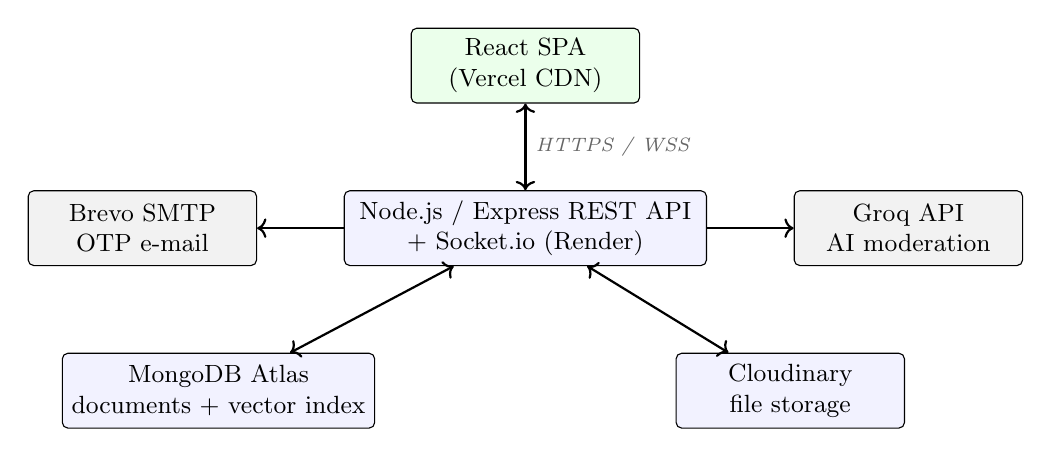
\begin{tikzpicture}[
  node distance=0.55cm and 1.1cm,
  box/.style={draw, rounded corners=2pt, align=center, font=\small,
              minimum height=0.95cm, minimum width=2.9cm, fill=blue!5},
  ext/.style={draw, rounded corners=2pt, align=center, font=\small,
              minimum height=0.95cm, minimum width=2.9cm, fill=gray!10},
  lbl/.style={font=\scriptsize\itshape, text=black!60},
  arr/.style={-{Stealth[length=2.5mm]}, thick}]

  \node[box, fill=green!8] (react) {React SPA\\(Vercel CDN)};
  \node[box, below=1.1cm of react, minimum width=4.6cm]
       (api) {Node.js / Express REST API\\+ Socket.io (Render)};
  \node[box, below left=1.1cm and -0.4cm of api] (mongo)
       {MongoDB Atlas\\documents + vector index};
  \node[box, below right=1.1cm and -0.4cm of api] (cloud)
       {Cloudinary\\file storage};
  \node[ext, right=of api] (groq) {Groq API\\AI moderation};
  \node[ext, left=of api] (brevo) {Brevo SMTP\\OTP e-mail};

  \draw[arr, <->] (react) -- node[lbl, right]{HTTPS / WSS} (api);
  \draw[arr, <->] (api) -- (mongo);
  \draw[arr, <->] (api) -- (cloud);
  \draw[arr, ->] (api) -- (groq);
  \draw[arr, ->] (api) -- (brevo);
\end{tikzpicture}
\caption{Three-tier system architecture of Campus Resource Hub}
\label{fig:arch}
\end{figure}

\subsection{System Workflow}
Figure~\ref{fig:workflow} shows the complete system workflow. After
OTP-verified signup and JWT login, users reach a role-aware
dashboard from which all eleven functional flows branch out:
resources, events, clubs, lost-and-found, announcements, chat,
notifications, AI search, admin panel, and profile management. The
central design pattern shared by all content flows is
\emph{create $\rightarrow$ AI scan $\rightarrow$ moderator approval
$\rightarrow$ publish $\rightarrow$ notify}.

\reportfig[0.95]{workflow.png}{Overall system workflow (exported
from the project's Lucidchart/draw.io diagram)}{fig:workflow}

\subsection{User Roles}
Access control follows a three-tier role model. Table~\ref{tab:roles}
summarizes what each role is allowed to do; every privileged API
route enforces these rules through the \texttt{authorize} middleware.
\begin{table}[htbp]
\centering
\caption{User roles and their permissions}
\label{tab:roles}
\begin{tabular}{@{}p{2.4cm}p{11cm}@{}}
\toprule
\textbf{Role} & \textbf{Permissions} \\
\midrule
Student & Browse/search all published content; upload resources;
          post lost-and-found items; RSVP to events; join clubs;
          chat; rate and download resources; manage own profile. \\
Moderator & All student permissions, plus: approve/reject resources,
          events, announcements, and lost-and-found posts; review
          AI-flagged items; create events, clubs, and announcements;
          block/unblock users. \\
Admin & All moderator permissions, plus: change user roles; delete
          users; full platform statistics. \\
\bottomrule
\end{tabular}
\end{table}

\section{Technology Stack}
The complete technology stack is listed in Table~\ref{tab:stack}.
All layers use JavaScript, which keeps the codebase uniform and
allows shared conventions between frontend and backend.
\begin{table}[htbp]
\centering
\caption{Technology stack of Campus Resource Hub}
\label{tab:stack}
\begin{tabular}{@{}llp{6.4cm}@{}}
\toprule
\textbf{Layer} & \textbf{Technology} & \textbf{Purpose} \\
\midrule
Frontend & React 18 + Vite & Single-page application UI \\
         & React Router & Client-side routing, protected routes \\
Backend  & Node.js + Express 5 & REST API server \\
         & Socket.io & Real-time messaging and notifications \\
Database & MongoDB Atlas + Mongoose & Document storage, schemas,
           indexes \\
         & Atlas Vector Search & 384-dim semantic search index \\
AI       & Groq LLM API & Content-safety moderation \\
         & Transformers.js (MiniLM) & Local sentence-embedding
           generation \\
Storage  & Cloudinary & File and image hosting \\
Auth     & JWT + bcrypt & Stateless sessions, password hashing \\
E-mail   & Brevo SMTP + Nodemailer & OTP delivery \\
Hosting  & Vercel / Render & Frontend CDN / backend server \\
\bottomrule
\end{tabular}
\end{table}

\section{Database Design}
The database consists of eleven MongoDB collections. Their fields
and relationships are shown in the entity--relationship diagram
(Figure~\ref{fig:erd}) and summarized in
Table~\ref{tab:collections}. The \texttt{User} collection is the
hub: nearly every other collection references it. All content
collections share a common moderation sub-document
(\texttt{approved}, \texttt{approvedBy}, \texttt{rejectionReason},
AI verdict), which keeps the approval workflow uniform across
modules.

\reportfig[0.95]{erd.png}{Entity--relationship diagram of the
eleven MongoDB collections (exported from draw.io)}{fig:erd}

\begin{table}[htbp]
\centering
\caption{Summary of database collections}
\label{tab:collections}
\begin{tabular}{@{}lp{9.6cm}@{}}
\toprule
\textbf{Collection} & \textbf{Purpose and key fields} \\
\midrule
User & Account data: name, unique e-mail and student ID,
  department, role, bcrypt-hashed password, block status. \\
AuthOtp & Hashed signup / password-reset OTPs with TTL index for
  automatic expiry. \\
Resource & Study material metadata: course, department, semester,
  file info, Cloudinary IDs, moderation verdict, downloads, rating. \\
Announcement & Notice content, priority, scheduled
  \texttt{publishAt}, expiry, read receipts, attachments. \\
Event & Date/time/location, capacity (0 = unlimited), RSVP
  registrations (going / maybe / declined), club reference. \\
Club & Name, category, join policy (open / request), members with
  roles (member / officer), pending join requests. \\
LostFoundItem & Item type (lost / found), private contact info,
  claim list with statuses, resolution timestamps. \\
Conversation & Direct or group chat thread: members, admins, last
  message reference. \\
Message & Sender, text, attachments, reply reference, delivered-to
  and seen-by lists. \\
Notification & Per-user feed entries with type, link, and read
  flag. \\
Embedding & 384-dimensional vector, source type + ID (polymorphic),
  content hash to skip unnecessary re-embedding. \\
ResourceChunk & Ordered text or safe-image-description passage,
  parent resource, passage type, and 384-dimensional embedding. \\
\bottomrule
\end{tabular}
\end{table}

\section{API Design}
The REST API is organized into nine route groups, protected by two
middleware layers: \texttt{protect} (JWT verification) and
\texttt{authorize} (role check).

\begin{table}[htbp]
\centering
\caption{REST API route groups (representative endpoints)}
\label{tab:api}
\begin{tabular}{@{}llp{6.6cm}@{}}
\toprule
\textbf{Group} & \textbf{Base path} & \textbf{Representative operations} \\
\midrule
Auth & \texttt{/api/auth} & signup, verify-signup-otp, login,
  forgot/reset password, profile update \\
Resources & \texttt{/api/resources} & upload, list/filter, preview,
  file stream, download count, rate \\
Announcements & \texttt{/api/announcements} & create, approve, pin,
  mark read, attachment stream \\
Events & \texttt{/api/events} & create, approve, register, RSVP
  update, cancel \\
Clubs & \texttt{/api/clubs} & create, join/leave, decide request,
  set member role \\
Lost-Found & \texttt{/api/lost-found} & post, claim, decide claim,
  resolve, reopen \\
Chat & \texttt{/api/chat} & conversations, messages, group
  management, AI assistant (stream) \\
Notifications & \texttt{/api/notifications} & list, mark read,
  clear \\
Admin & \texttt{/api/admin} & statistics, user list, role change,
  block, delete \\
\bottomrule
\end{tabular}
\end{table}

\section{Security Design}
Security measures are applied at every layer:
\begin{itemize}[itemsep=2pt]
  \item \textbf{Account security}: e-mail ownership proven by OTP
        before account creation; OTPs stored only as hashes with
        automatic TTL expiry and attempt counting; passwords hashed
        with bcrypt (salt rounds = 10).
  \item \textbf{Transport / headers}: HTTPS everywhere, Helmet
        security headers, strict CORS allow-list.
  \item \textbf{Abuse prevention}: express-rate-limit (1{,}500
        requests per 15 minutes per IP); upload size and type
        validation with Multer.
  \item \textbf{Authorization}: JWT verification middleware plus
        role checks on every privileged route; chat access verified
        per conversation membership.
  \item \textbf{Content safety}: AI moderation scan on every upload;
        flagged items quarantined; human approval required before
        anything is published.
  \item \textbf{Privacy}: lost-and-found contact details hidden by
        default and revealed only to approved claimants; passwords
        excluded from all API responses.
\end{itemize}

% ------------------------------------------------------------
\chapter{Implementation Overview}
% ------------------------------------------------------------
After a successful login, every user lands on a role-aware dashboard
(Figure~\ref{fig:dashboard}) that summarizes platform activity ---
total resources, announcements, upcoming events, and open
lost-and-found items --- and provides quick access to recent
resources and the latest announcements. The persistent left
navigation and the top ``Ask AI'' search bar are available from
every page.

\reportfig{dashboard.png}{Role-aware dashboard with activity summary
cards, recent resources, and latest announcements}{fig:dashboard}

\section{Authentication and OTP Verification}
Signup collects name, e-mail, student ID, department, and password.
The server generates a six-digit OTP, stores its hash in the
\texttt{AuthOtp} collection with a TTL expiry, and e-mails it via
Brevo SMTP. Only after correct OTP entry is the account created with
the default \texttt{student} role. Login returns a signed JWT; a
parallel OTP flow handles forgotten passwords.

\reportfig{auth-login.png}{Login and signup with e-mail OTP
verification}{fig:auth}

\section{Resource Upload and AI Moderation Pipeline}
Upload accepts PDF, DOCX, PPTX, XLSX, and images with course,
department, and semester metadata. The file goes to Cloudinary;
text and images are then extracted server-side (pdf-parse, Mammoth,
canvas) and scanned through a provider chain: Groq first, Hugging
Face second, and OpenAI last. Clean, fully inspected uploads are
published automatically. Flagged files, partial extractions, and
provider-unavailable checks fail safely into the moderator review
queue; they are never auto-published. Rejection notifies the uploader
with a reason. Searchable passages are generated asynchronously for
approved text and safe image descriptions.

\reportfig{resource-upload.png}{Resource upload with metadata and
moderation status}{fig:upload}
\reportfig{resource-browse.png}{Browsing, filtering, previewing and
rating published resources}{fig:browse}

\section{Events with Capacity-Aware RSVP}
Moderators create events with date, time, location, and optional
capacity. Students RSVP as \emph{going}, \emph{maybe}, or
\emph{declined}; registration is blocked once capacity is reached.
Users see their events in a calendar view, and posters or admins can
cancel events, which notifies registrants.

\reportfig{events.png}{Event listing and RSVP flow}{fig:events}

\section{Clubs with Join Policies and Member Roles}
Each club declares a join policy: \emph{open} (instant membership)
or \emph{request} (application with an optional note, decided by an
officer or the creator). Members hold \emph{member} or
\emph{officer} roles; officers manage requests and membership.

\reportfig{clubs.png}{Club directory and membership
management}{fig:clubs}

\section{Lost and Found with Claim Workflow}
Users post lost or found items with photos. Contact information is
hidden by default. Another user files a claim with a note; the
poster (or a moderator) approves or rejects it. Approval reveals
contact details to the claimant only and moves the item to
\emph{claimed}, then \emph{resolved}. This protects personal data
while still reuniting items with owners.

\reportfig{lostfound.png}{Lost-and-found listing and claim
dialog}{fig:lostfound}

\section{Announcements with Scheduled Publishing}
Announcements carry a priority (normal / important / urgent),
optional attachments, a scheduled \texttt{publishAt} time, and an
optional expiry. A server-side scheduler publishes each announcement
exactly once at its scheduled time and broadcasts a notification.
Read receipts record which students have seen each notice.

\reportfig{announcements.png}{Announcement feed with priority
badges}{fig:announcements}

\section{Real-Time Chat}
Chat supports direct and group conversations over Socket.io.
Messages support attachments, replies, and editing; the system
tracks per-user delivery and seen status. Group admins can rename
groups, add or remove members, and promote other admins. All chat
REST endpoints re-verify conversation membership server-side.

\reportfig{chat.png}{Real-time direct and group messaging with seen
receipts}{fig:chat}

\section{Notifications}
Every significant action --- new message, approved or rejected
upload, event change, claim decision, announcement --- creates a
notification document and pushes it live over Socket.io. The bell
menu supports mark-as-read, mark-all, and clear.

\section{Semantic Search and AI Assistant}
When content is published, its title and body are embedded with a
multilingual MiniLM sentence-transformer running inside the Node
process (Transformers.js); the 384-dimensional unit vector is stored
in the \texttt{Embedding} collection, one shared collection for all
five content types. A content hash prevents redundant re-embedding
when text has not changed. Queries embed the user's question and run
Atlas \texttt{\$vectorSearch}; results are re-checked against each
source collection's visibility rules, so search can never leak
unpublished content. The AI assistant wraps this pipeline and
streams its answer token-by-token over server-sent events. The
assistant is reachable from the ``Ask AI about resources'' bar at the
top of every page (visible in Figure~\ref{fig:dashboard}).

For resource files, extracted text and safe image descriptions are
split into overlapping ordered chunks and embedded separately in the
\texttt{ResourceChunk} collection. Retrieval first applies the
current user's resource-visibility filter, then ranks matching
passages and metadata together. The assistant can therefore answer
questions about what a PDF contains, summarize a DOCX file, or
describe an indexed image while citing numbered, clickable source
cards. Exact-title and lexical-passage matches outrank weaker legacy
semantic matches.

\section{Admin Panel}
The panel shows platform statistics (users, resources, pending
approvals), a user-management table (block/unblock, delete, role
change --- role change restricted to admins), and approval queues
for every content type including AI-flagged items.

\reportfig{admin.png}{Admin panel: statistics and approval
queues}{fig:admin}

\section{Deployment}
The frontend is deployed on Vercel (global CDN, automatic builds).
The backend runs on Render with environment-based configuration;
\texttt{dns.setDefaultResultOrder("ipv4first")} works around the
host's missing IPv6 egress route. MongoDB Atlas hosts the database
and the vector search index; Cloudinary stores all files. The whole
stack currently runs on free tiers.

% ------------------------------------------------------------
\chapter{Result \& Analysis}
% ------------------------------------------------------------
\section{Achieved Features}
All objectives set in Chapter 1 were implemented and verified
manually across the three roles:

\begin{table}[htbp]
\centering
\caption{Feature completion summary}
\label{tab:results}
\begin{tabular}{@{}p{5.2cm}p{8.2cm}@{}}
\toprule
\textbf{Feature} & \textbf{Status / observed behaviour} \\
\midrule
OTP signup \& JWT login & Accounts created only after correct OTP;
  expired OTPs auto-deleted by TTL index. \\
Resource sharing & Upload, preview, download, rating and view
  counting work for all five file types. \\
AI moderation & Harmful, partially inspected, or provider-unavailable
  uploads are quarantined; clean fully inspected files auto-publish. \\
Approval workflow & Uniform across resources, events, announcements
  and lost-and-found; rejection reasons delivered as
  notifications. \\
Events & Capacity limit enforced at registration time; RSVP status
  editable; calendar view correct. \\
Clubs & Open clubs join instantly; request clubs require officer
  decision; roles enforced. \\
Lost \& found & Contact hidden until claim approval; item lifecycle
  open $\rightarrow$ claimed $\rightarrow$ resolved. \\
Chat & Real-time delivery with delivered/seen receipts; group
  administration functions. \\
Semantic search & Meaning-based matches returned with sources; AI
  assistant streams answers. \\
Admin panel & Statistics, user management and all approval queues
  operational. \\
\bottomrule
\end{tabular}
\end{table}

\section{Security Analysis}
The two-layer moderation pipeline proved effective in testing:
AI-flagged uploads never became publicly visible, while clean and
fully inspected uploads were auto-published. Partial extraction or
provider failure sent content to human review instead of failing
open. Rate limiting blocked request floods with HTTP 429 responses.
JWT tampering attempts were
rejected by signature verification, and role-guarded endpoints
returned HTTP 403 for insufficient roles. Lost-and-found contact
details were confirmed to be absent from API responses until a claim
was approved.

\section{Bug Report and Resolution Log}
The Git history of both repositories was reviewed to distinguish
implemented fixes from planned work. Table~\ref{tab:buglog} records
the principal defects that affected safety, search correctness,
real-time connectivity, or usability. Commit hashes provide
traceable implementation evidence; merged pull requests represent
the authoritative state on the \texttt{main} branches.

\begin{longtable}{@{}>{\raggedright\arraybackslash}p{1.15cm}
  >{\raggedright\arraybackslash}p{4.15cm}
  >{\raggedright\arraybackslash}p{5.15cm}
  >{\raggedright\arraybackslash}p{3.1cm}@{}}
\caption{Resolved defect log derived from Git history and regression tests}
\label{tab:buglog}\\
\toprule
\textbf{ID} & \textbf{Observed defect and impact} &
\textbf{Root cause and implemented resolution} &
\textbf{Evidence / status} \\
\midrule
\endfirsthead
\toprule
\textbf{ID} & \textbf{Observed defect and impact} &
\textbf{Root cause and implemented resolution} &
\textbf{Evidence / status} \\
\midrule
\endhead
BR-01 & Graphic, adult, or otherwise unsafe files could be approved
when a vision provider failed or only part of a document was
extracted. This was the highest-severity publication risk. &
The earlier path treated incomplete inspection too optimistically.
Moderation now fails safe: flagged, partial, and provider-unavailable
results remain unpublished for human review. Deterministic text
screening and the Groq--Hugging Face--OpenAI provider order were also
added. & \texttt{df5fa96}; four moderation-policy regression tests
pass. Resolved. \\
\addlinespace
BR-02 & The AI assistant could find a resource by title but could not
reliably explain what was inside its PDF or Office document. &
Only short metadata and a limited excerpt were searchable. The first
repair stored file excerpts (\texttt{d356801}); the completed repair
adds ordered overlapping \texttt{ResourceChunk} passages, embeddings,
safe image descriptions, and an existing-resource backfill. &
\texttt{d356801}, \texttt{0e707b3}; 54 approved resources indexed
with zero extraction failures. Resolved. \\
\addlinespace
BR-03 & Content questions could rank weakly related legacy semantic
matches above an exact title or file-passage match, producing noisy
sources. &
Metadata and passage relevance had comparable scores. The final
hybrid rank gives exact titles and lexical file passages stronger
weight, loads ordered passages for summary intent, and preserves
inline source numbering. & \texttt{0e707b3}; real PDF-summary and
deadlock-query checks place the relevant Operating Systems resources
first. Resolved. \\
\addlinespace
BR-04 & A semantic/vector result risked bypassing the visibility rules
used by ordinary keyword queries. &
Vector candidates were not sufficient authorization evidence. Every
candidate is now joined back through the same approved/owner/role
filter before its passages are exposed. & \texttt{c755663},
\texttt{0e707b3}; streaming test returned zero unauthorized sources.
Resolved. \\
\addlinespace
BR-05 & Real-time chat connections were unreliable after frontend
deployment on Vercel. &
The Socket.io client transport did not match the deployed network
path. The client now prefers explicit WebSocket transport with
deployment-compatible connection settings. & \texttt{42ef620}; fix
merged to frontend \texttt{main}. Resolved. \\
\addlinespace
BR-06 & Expanding the header AI input to multiple lines changed the
header height and obscured adjacent controls; an interim revert also
removed desired behavior. &
The textarea participated in normal header layout. It now grows in an
absolutely positioned layer, retains Enter/Shift+Enter behavior, and
shows readable Markdown plus numbered source cards. &
\texttt{757141d}, \texttt{f4259f7}, \texttt{16edb5f},
\texttt{641b1bc}; production build passes. Resolved. \\
\bottomrule
\end{longtable}

\subsection{Current Verification Snapshot}
After the final fixes, the backend unit suite completed with six of
six tests passing. End-to-end API checks covered a PDF summary, a
topic question across resources, an indexed-image question, and the
server-sent-event completion path. The authorization regression test
returned eight visible sources and zero unauthorized sources. The
frontend production bundle compiled successfully. Browser automation
was not part of this snapshot because the dedicated local browser
runner was unavailable; this is a tooling limitation, not evidence of
a product failure.

\subsection{Open Operational Constraint}
Vision indexing depends on third-party quotas. During the verification
run, graphic-image moderation succeeded, but Groq reached a temporary
rate limit and the Hugging Face and OpenAI accounts reported exhausted
credits. The application handles this condition safely: it does not
auto-publish unverified content, and the configured fallback order is
retained for the next available provider. This constraint should be
monitored separately from functional defects in the application.

\section{Performance and Capacity Analysis}
The deployment currently runs entirely on free tiers, which defines
its capacity envelope (Table~\ref{tab:capacity}).

\begin{table}[htbp]
\centering
\caption{Capacity analysis of the current free-tier deployment}
\label{tab:capacity}
\begin{tabular}{@{}p{4.4cm}p{4.2cm}p{4.6cm}@{}}
\toprule
\textbf{Component} & \textbf{Limit} & \textbf{Practical effect} \\
\midrule
Render web service (free) & 512 MB RAM, 0.1 vCPU & Main bottleneck;
  AI scan + embedding jobs are CPU-heavy \\
MongoDB Atlas M0 & $\sim$100 ops/s, 500 connections & Caps
  simultaneous active users at $\sim$100 \\
Socket.io connections & Few KB per idle socket & Hundreds of idle
  users are unproblematic \\
Cloudinary free tier & Monthly bandwidth credits & Long-term quota,
  not a concurrency limit \\
\bottomrule
\end{tabular}
\end{table}

In practice the platform comfortably serves \textbf{50--100
concurrent active users} (department scale) and can hold
\textbf{200--300 logged-in connections} including idle users.
Load beyond that first saturates the 0.1 vCPU during simultaneous
uploads (each triggering an AI scan and embedding generation), then
the Atlas M0 operation ceiling. An inexpensive upgrade path ---
Render Starter (\$7/month) plus Atlas M10 --- raises the envelope to
500+ active users, sufficient for full-campus rollout.

\section{Cost Efficiency}
The entire system runs at \textbf{zero recurring cost} on free
tiers, using Vercel (frontend), Render (backend), MongoDB Atlas M0
(database + vector search), Cloudinary (storage), Brevo (300
e-mails/day), and Groq (moderation API). This makes the platform
immediately viable for a university without a software budget.

% ------------------------------------------------------------
\chapter{Future Enhancements}
% ------------------------------------------------------------
Planned improvements include:
\begin{enumerate}[itemsep=2pt]
  \item \textbf{Mobile application} --- a React Native client
        sharing the existing REST/Socket.io backend.
  \item \textbf{Background job queue} --- moving AI scanning and
        embedding generation off the request path (e.g.\ BullMQ) to
        remove the largest CPU spike.
  \item \textbf{Push notifications} --- Web Push / FCM so users are
        reachable when the site is closed.
  \item \textbf{Richer analytics} --- per-department dashboards,
        trending resources, and event attendance reports.
  \item \textbf{Federated login} --- university e-mail SSO (OAuth2)
        alongside OTP signup.
  \item \textbf{Horizontal scaling} --- multiple backend instances
        with a Socket.io Redis adapter once campus-wide load
        requires it.
  \item \textbf{Accessibility and localization} --- full Bangla
        interface and WCAG-compliant UI review.
\end{enumerate}

% ------------------------------------------------------------
\chapter{Conclusion}
% ------------------------------------------------------------
This project set out to replace the fragmented, unmoderated channels
through which campus information currently flows with a single,
secure, intelligent platform. The delivered system --- Campus
Resource Hub --- implements verified onboarding, a categorized and
rated study-resource repository, capacity-aware events, club
management, a privacy-preserving lost-and-found process, scheduled
announcements, real-time messaging, and a semantic AI assistant, all
protected by a uniform two-layer moderation pipeline and role-based
access control. The implementation demonstrates that modern
techniques usually associated with large commercial platforms ---
AI content moderation, vector-based semantic search, streamed LLM
assistance --- can be integrated into a student project deployed
entirely on free cloud tiers. Capacity analysis confirms the current
deployment already serves a department-sized community, with a clear
and inexpensive path to campus scale. Beyond its immediate utility,
the project provided deep practical experience in full-stack
architecture, real-time systems, applied AI services, and cloud
deployment.

% ------------------------------------------------------------
% REFERENCES
% ------------------------------------------------------------
\begin{thebibliography}{9}
\addcontentsline{toc}{chapter}{References}

\bibitem{react} Meta Platforms, ``React -- The library for web and
native user interfaces,'' \url{https://react.dev}, accessed 2026.

\bibitem{express} OpenJS Foundation, ``Express -- Node.js web
application framework,'' \url{https://expressjs.com}, accessed 2026.

\bibitem{mongodb} MongoDB Inc., ``MongoDB Atlas Vector Search
documentation,''
\url{https://www.mongodb.com/docs/atlas/atlas-vector-search/},
accessed 2026.

\bibitem{socketio} Socket.io, ``Socket.io documentation,''
\url{https://socket.io/docs/}, accessed 2026.

\bibitem{sbert} N.~Reimers and I.~Gurevych, ``Sentence-BERT:
Sentence Embeddings using Siamese BERT-Networks,'' in
\textit{Proceedings of EMNLP-IJCNLP}, 2019.

\bibitem{minilm} W.~Wang et al., ``MiniLM: Deep Self-Attention
Distillation for Task-Agnostic Compression of Pre-Trained
Transformers,'' in \textit{Advances in Neural Information Processing
Systems (NeurIPS)}, 2020.

\bibitem{jwt} M.~Jones, J.~Bradley, and N.~Sakimura, ``JSON Web
Token (JWT),'' RFC 7519, IETF, 2015.

\bibitem{cloudinary} Cloudinary Ltd., ``Cloudinary developer
documentation,'' \url{https://cloudinary.com/documentation},
accessed 2026.

\bibitem{moodle} Moodle HQ, ``Moodle -- Open-source learning
platform,'' \url{https://moodle.org}, accessed 2026.
\end{thebibliography}

\end{document}
